% Changing book to article will make the footers match on each page,
% rather than alternate every other.
%
% Note that the article class does not have chapters.
\documentclass[a4paper,9pt,twoside,twocolumn,openany]{book}

\usepackage[utf8]{inputenc}
\usepackage[OT2, T1]{fontenc}

% Use babel or polyglossia to automatically redefine macros for terms
% Armor Class, Level, etc...
% Default output is in English; captions are located in lib/dndstring-captions.sty.
% If no captions exist for a language, English will be used.
%1. To load a language with babel:
%	\usepackage[<lang>]{babel}
%2. To load a language with polyglossia:
%	\usepackage{polyglossia}
%	\setdefaultlanguage{<lang>}
\usepackage[french]{babel}
%usepackage[italian]{babel}
% For further options (multilanguage documents, hypenations, language environments...)
% please refer to babel/polyglossia's documentation.

\usepackage{lipsum}
\usepackage{listings}
\usepackage{swe}
\usepackage{pdfpages}
\usepackage{tikz}
\usepackage{xcolor} 
\definecolor{ultramarine}{RGB}{56,77,61}

\settoggle{justified}{true}
\justifying 

\lstset{%
  basicstyle=\ttfamily,
  language=[LaTeX]{TeX},
}

% Start document
\begin{document}

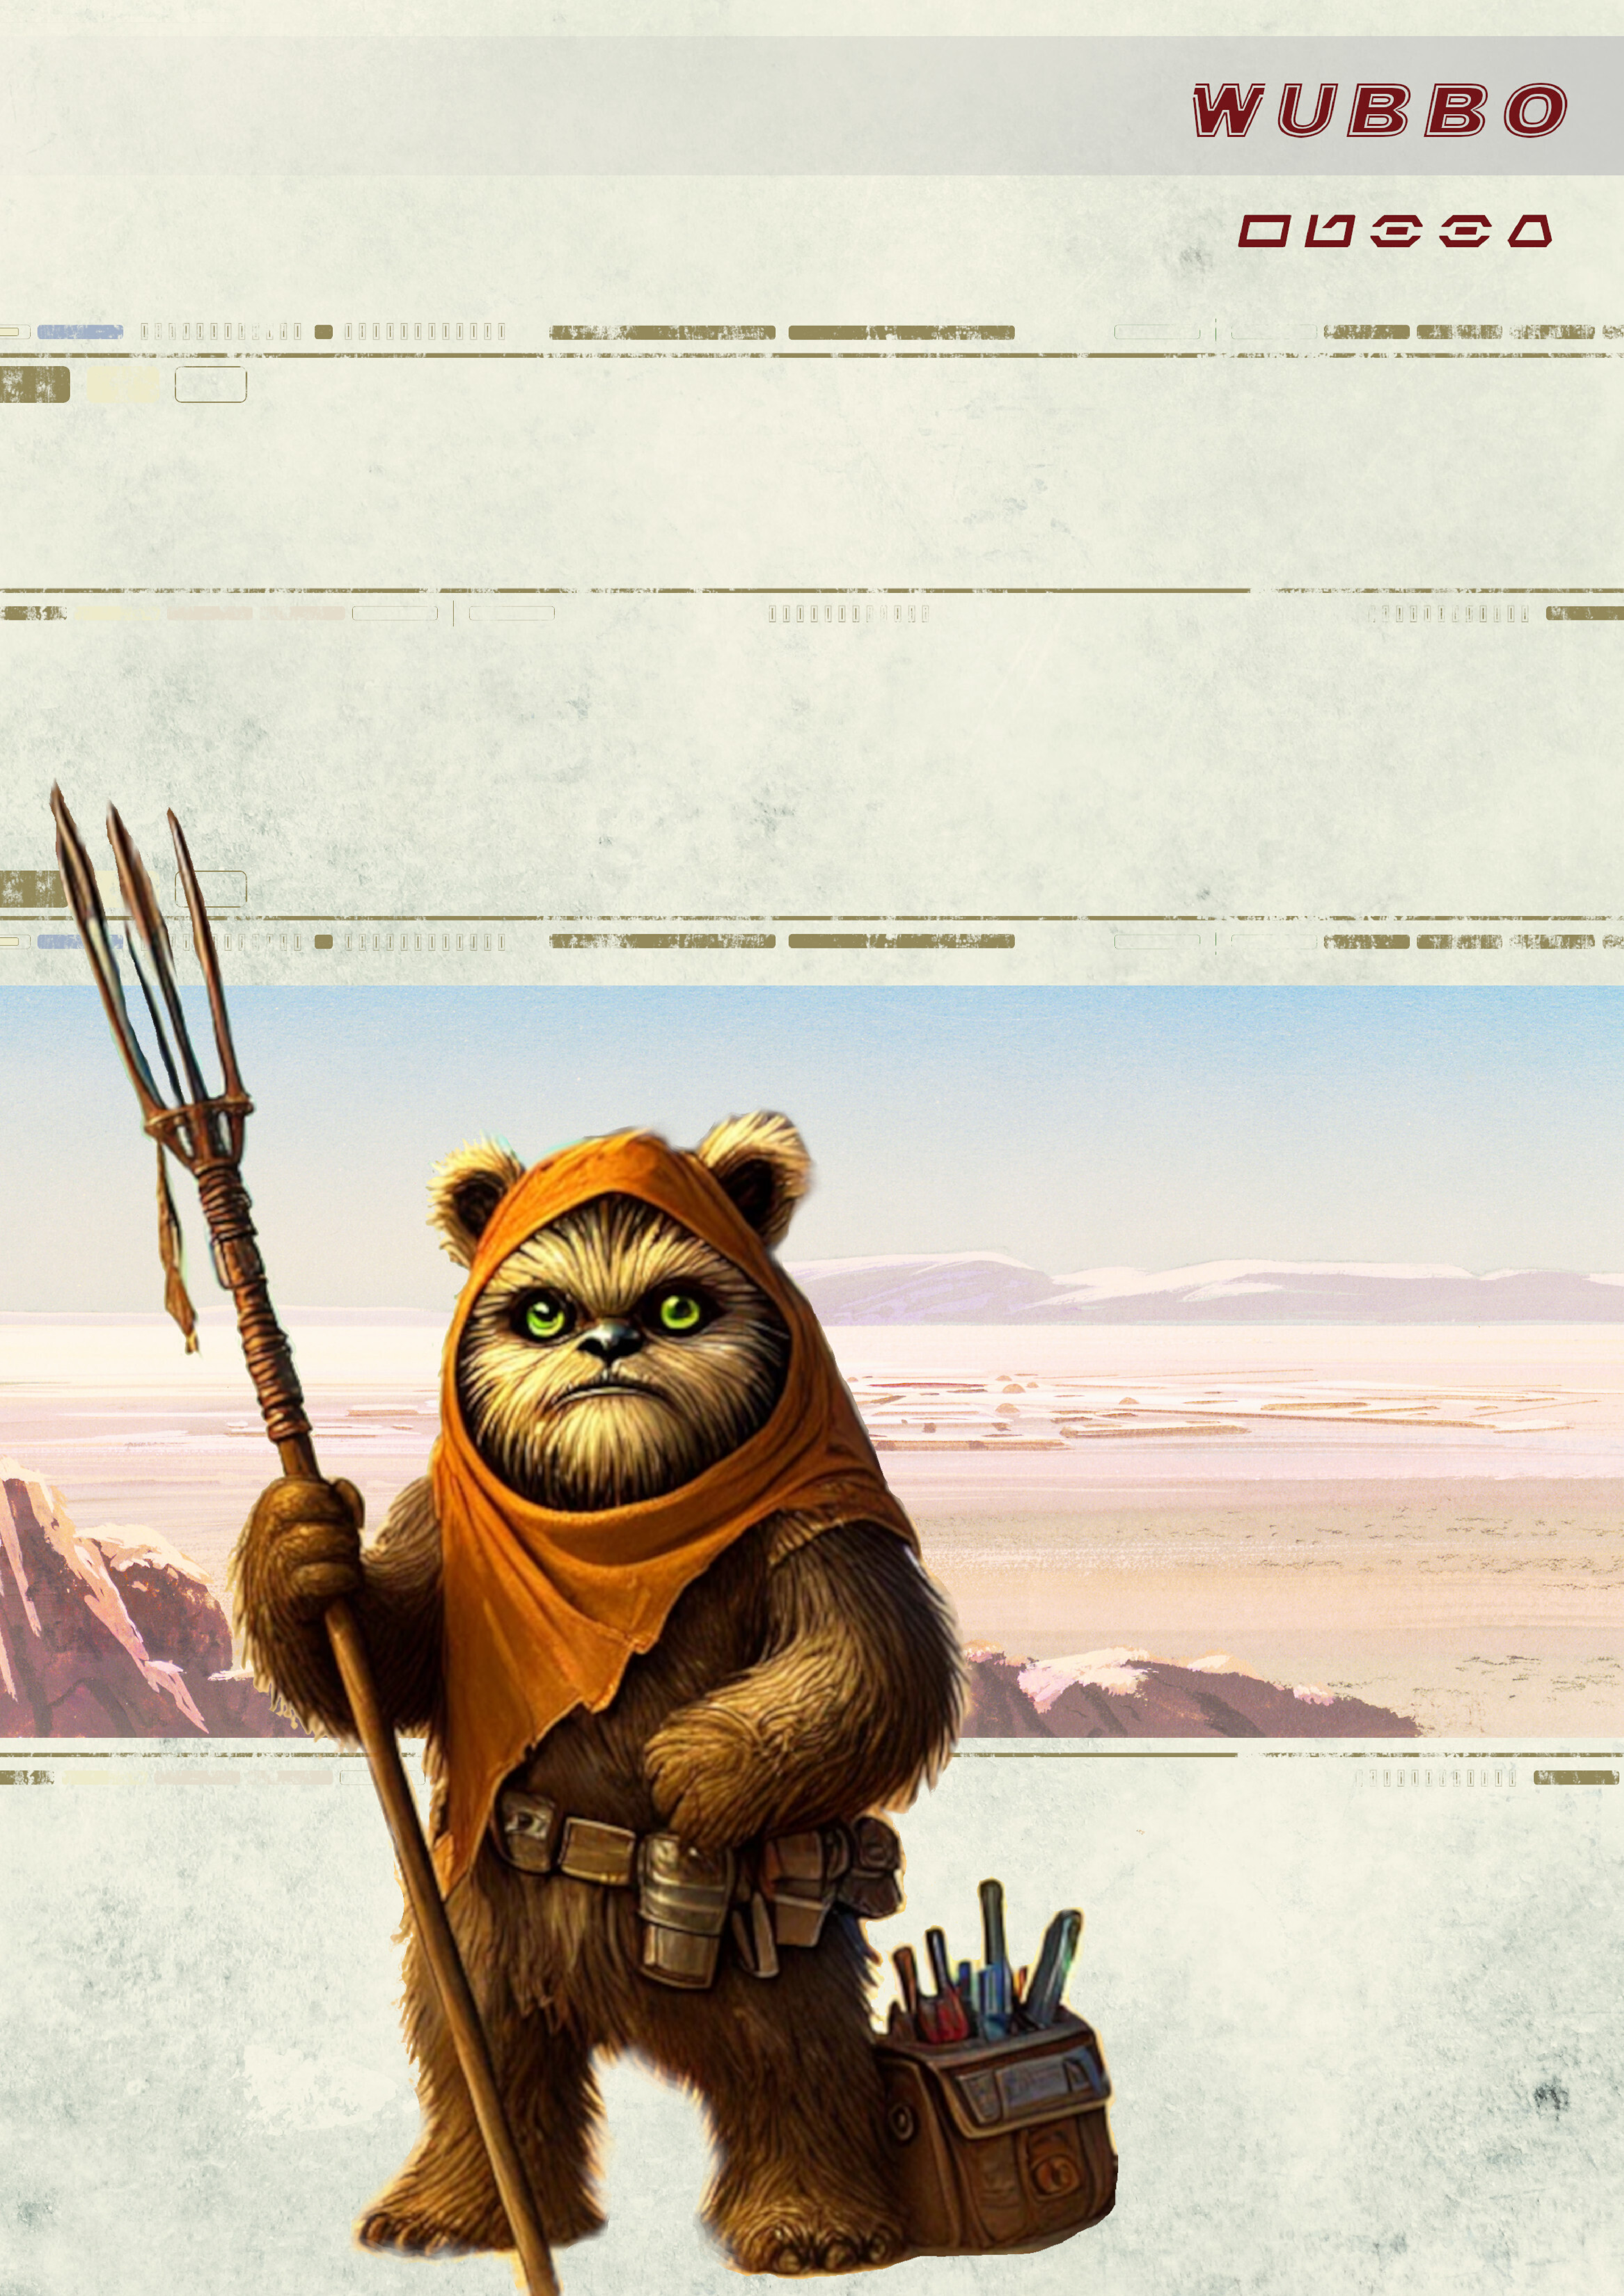
\includepdf[pages=1,%
    picturecommand*={%
    \put(30,800){ {\huge \scshape \textbf{ \sffamily\bfseries \color{ultramarine} Journal de Bord }} }%
}]{img/wubbo.pdf}

% Seconde de couverture

\chapter{Généralités et Crédits}

\section{Maître du jeu}

\paragraph{Pibeto} Empire, Résistance, Rebelles, Animaux, Ambiance, ... \emph{Merci à lui.}

\section{Joueurs}

Ce personnage est créé dans le cadre d'une seconde initiation au sein d'Airbus, en décembre 2024.

\section{Quelques aides et rappels}

\subsection{Investir}

\begin{dndtable}[p{0.3\columnwidth}X]
  \textbf{Achat}                & \textbf{Description} \\
  Compétence carrière           & 5 * seuil (5, 10, 15, ...) \\
  Compétence hors carrière      & 5 * seuil + 5 (5, 10, 15, ...) \\
  Arbre de spéc.                & 10 xp * nb. tot. specs. \\
  .... si nouvel                & Majoration de 10 xp \\
\end{dndtable}

\subsection{Symbolique}

\begin{dndtable}[cX]
  \textbf{Dés}                & \textbf{Description} \\
  \boost         & aide, bonus , \emph{boost} \\
  \setback       & contrainte, malus \\
  \difficulty    & difficulté \\
  \ability       & habilité \\
  \challenge     & challenge \\
  \proficiency   & efficacité \\
\end{dndtable}

\begin{dndtable}[cX]
  \textbf{Symbole}  & \textbf{Description} \\
  \successA & Succès \\
  \failureA & \'Echec \\
  \advantage    & Avantage \\
  \threat       & Menace \\
  \triumph   & Triomphe \\
  \despair   & Fumble \\
\end{dndtable}

\subsection{Capacités spéciales}
\paragraph{Petite taille} Les Ewoks sont généralement plus petits que la moyenne et comptent comme une silhouette 0. Ils commencent le jeu avec un rang dans Furtivité (Stealth) ou Survie (Survival). Cependant, ils ne peuvent pas dépasser le rang 2 dans l'une de ces compétences avant d'avoir dépensé de l'expérience pour améliorer leur carrière ou leur spécialisation.

\paragraph{Sens aiguisés} Les Ewoks ajoutent un \boost aux tests de Perception et de Vigilance.

\paragraph{Utilisateurs de technologie primitive} Les Ewoks augmentent la difficulté de tous les tests pour utiliser une technologie inconnue d’un rang de difficulté (\difficulty$\Rightarrow{}$\challenge). Cependant, s’ils passent une période prolongée à utiliser une pièce spécifique de technologie, ils peuvent se familiariser avec et être exemptés de cette règle (à la discrétion du MJ).
De plus, avec l’approbation du MJ, un joueur Ewok peut dépenser 10 XP pour supprimer définitivement ce désavantage de son personnage.

\newpage

\tableofcontents

\chapter{Le personnage}

\section{Wubbo}

\paragraph{\^Age} Temps humain … 42 ans
\paragraph{Sexe} Masculin
\paragraph{Race} Ewok

\subsection{Origines}

\begin{wrapfigure}{O}{0.25\textwidth}
    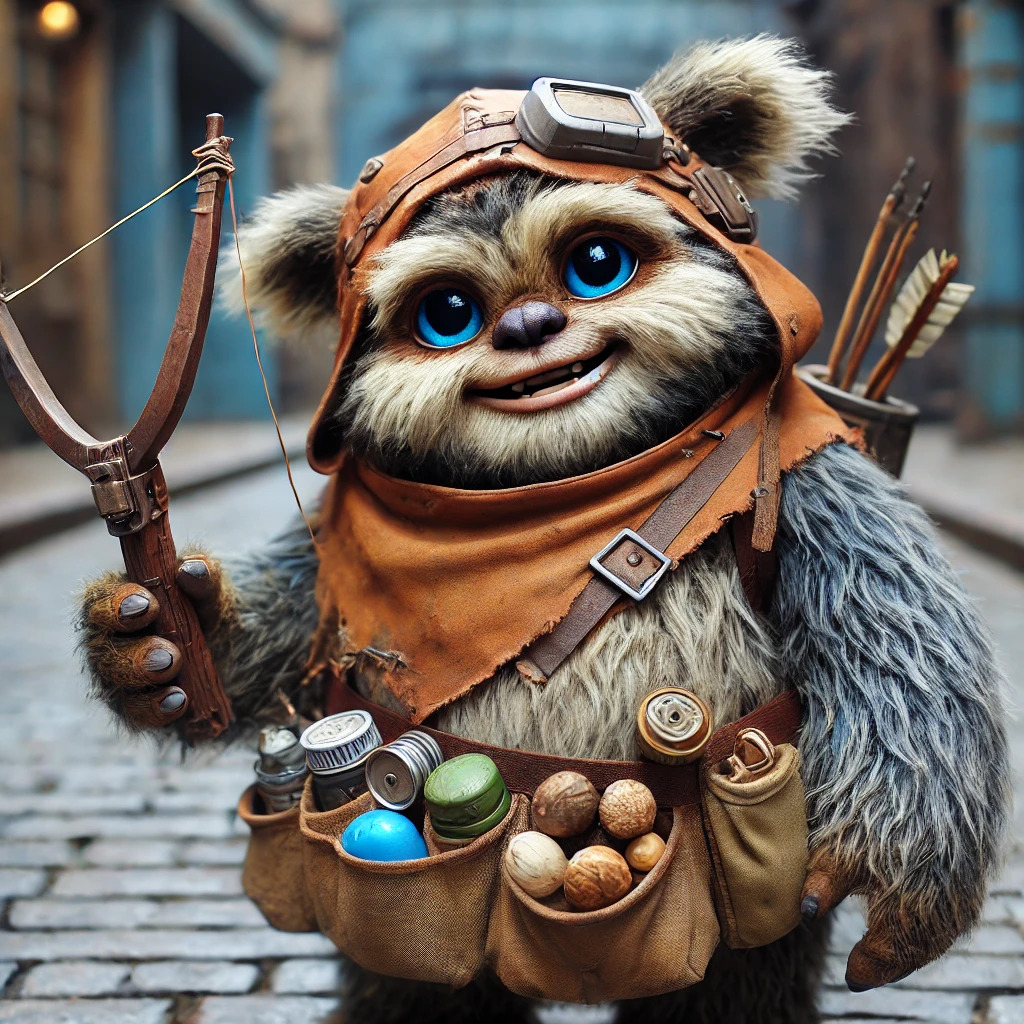
\includegraphics[width=0.25\textwidth]{img/ewok.jpg}
    \caption{Wubbo}
\end{wrapfigure}

Wubbo est né sur la lune forestière d’Endor, dans une petite tribu située à l’écart des autres villages Ewoks.
Très tôt, il a montré un esprit curieux et une fascination pour tout ce qui sortait de l’ordinaire : morceaux de métal abandonnés par les chasseurs, éclats de vaisseaux tombés, et parfois même les gadgets oubliés par les rebelles après la Bataille d’Endor.

Jeune, contrairement à ses camarades, qui se concentraient sur la chasse et la cueillette, votre Ewok aimait expérimenter.
Il fabriquait des pièges, bidouillait des objets rudimentaires, et testait des inventions, souvent au grand dam des anciens de sa tribu. Bien que ces expériences aient souvent causé des incidents, elles ont forgé sa créativité et son ingéniosité.

Un jour, il a découvert un morceau de technologie cassée – un générateur d’énergie miniature. Fasciné, il a essayé de le réparer, ce qui a provoqué une explosion mineure. Bien que personne n’ait été blessé, sa tribu l’a surnommé \emph{le casse-tou'}, un titre affectueux mais un peu moqueur.

\subsection{Compétences et personnalité}

\paragraph{Force} Débrouillard et rusé, il est un maître des outils improvisés.
Qu’il s’agisse de réparer une pièce d’un vaisseau ou de fabriquer un piège avec des branches, il trouve toujours une solution.

\paragraph{Faiblesse} Sa curiosité peut être dangereuse.
Il est parfois trop confiant et se retrouve dans des situations délicates en manipulant des objets ou en provoquant des ennemis.

\paragraph{Personnalité} Plein de bonne humeur, il adore les farces, même dans des moments critiques.
Mais derrière son apparence espiègle se cache un cœur loyal et une volonté de fer.

\section{La rencontre avec Salen Daro}

\subsection{Rêve d'Aventure}
Depuis son plus jeune âge, Wubbo rêvait de quitter les forêts denses d’Endor. Fasciné par les histoires des Rebelles et des voyageurs qui avaient visité sa lune natale, il se demandait constamment ce qui se trouvait au-delà des cimes des arbres. Le bruit des moteurs des vaisseaux traversant le ciel éveillait une curiosité inextinguible chez lui.

Malgré l’attachement de sa tribu à leurs traditions, Wubbo sentait qu’il n’était pas fait pour rester sur place. Il voulait voir la galaxie, rencontrer des gens différents, et vivre des aventures dignes des récits qui l’avaient bercé.

Un jour, il a pris une décision radicale : il rassemblerait ses quelques possessions (sa lance, sa fronde et quelques outils) et se faufilerait dans le premier vaisseau venu. Ce qu’il voulait, c’était partir — peu importait où.

\subsection{Une Rencontre Inattendue}
Un vieux cargo léger, \emph{L’Aube Furtive}, appartenant à un Twi’lek nommé \emph{Salen Daro}, faisait escale sur Endor pour livrer une cargaison discrète à un groupe de chasseurs. Profitant de l’agitation au spatioport improvisé, Wubbo, avec son habileté naturelle pour la furtivité, s’est glissé à bord du vaisseau.

Wubbo a trouvé refuge dans une caisse vide dans la soute. Lorsque le vaisseau a décollé, il a attendu plusieurs heures avant de sortir de sa cachette, attiré par les bruits intrigants du moteur et les odeurs nouvelles.

\paragraph{La découverte} Salen a découvert Wubbo en train d'explorer curieusement les couloirs du vaisseau. Plutôt que de réagir violemment, Salen, amusé et intrigué par ce petit passager clandestin, a entamé une discussion.

\subsection{Pourquoi Salen l’a gardé à bord}
Salen, bien qu’un peu cynique par nature, a un faible pour les créatures marginales et les âmes perdues. Après avoir discuté avec Wubbo, il a compris que l’Ewok n’avait aucune mauvaise intention : il cherchait juste à explorer la galaxie.

Wubbo, de son côté, a exprimé son admiration pour le pilote et le vaisseau. Avec ses yeux verts et or pétillants de curiosité, il a rapidement charmé Salen, qui voyait en lui un compagnon inattendu et attachant.

\subsection{Une Relation Gagnant-Gagnant}
Wubbo, bien que maladroit avec la technologie avancée, s’est montré très utile :
\begin{itemize}
    \item Il aidait Salen à réparer des composants mécaniques simples, souvent avec des idées ingénieuses inspirées de sa vie primitive.
    \item Sa petite taille et sa furtivité faisaient de lui un excellent éclaireur ou infiltreur lorsque le duo se trouvait dans des situations risquées.
    \item Surtout, il apportait une touche de joie et d’aventure à la vie de Salen, parfois trop monotone ou dangereuse.
\end{itemize}

En échange, Salen a enseigné à Wubbo les bases de la navigation spatiale, les dangers de la galaxie, et les subtilités du commerce (légal ou non). Peu à peu, leur relation s’est transformée en une amitié profonde, fondée sur la loyauté et le respect mutuel.

\subsection{Conclusion}
Wubbo considère Salen comme son premier véritable ami en dehors d’Endor et s’est juré de lui être fidèle en toutes circonstances. Pour Salen, Wubbo est plus qu’un passager : il est un compagnon fidèle qui lui rappelle pourquoi il a choisi cette vie d’aventurier.

Leur duo improbable forme une équipe pleine de contrastes, mais aussi d’ingéniosité et de bonne humeur, toujours prête à affronter les périls de la galaxie.

\section{Motivation}

Wubbo aspire à découvrir la galaxie et à vivre des aventures palpitantes, mais il reste profondément attaché aux valeurs d’amitié et de loyauté. À travers ses voyages, il espère non seulement s’émerveiller des mondes inconnus, mais aussi prouver qu’un Ewok peut être un compagnon de valeur dans un univers bien plus vaste que sa forêt natale.

\chapter{L'aventure}

\section{Une nouvelle équipe}
\subtitle{?? décembre 2024}


\clearevenpage

% Création de la quatrième de couverture
\onecolumn
\Large

\centering

\vfill

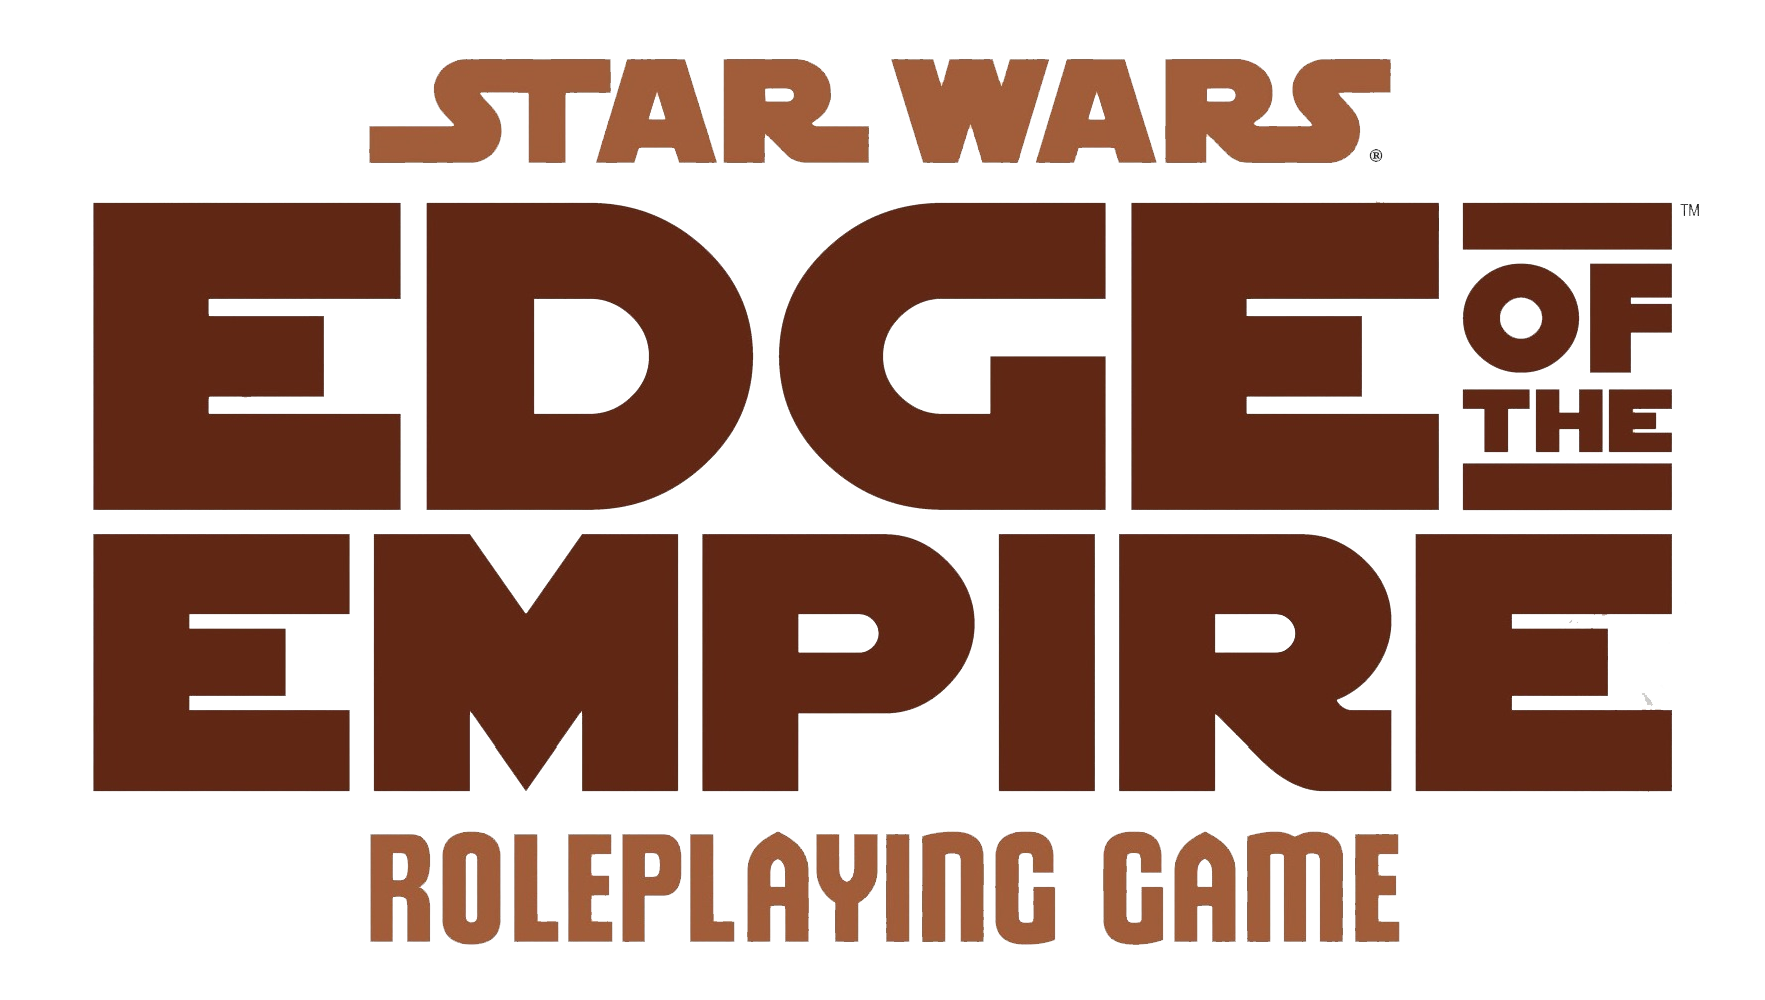
\includegraphics[width=1\textwidth]{img/SWEotE}


\vfill

L'histoire de quelques gars et demoiselles à travers l'espace.
\vfill

% End document
\end{document}
